\documentclass{article}

\usepackage{graphicx}
\usepackage{tikz}
\usepackage{tikzsymbols}
\usetikzlibrary{calc,patterns,shapes.geometric}
\pagestyle{empty}
\usepackage[margin=0pt]{geometry}
\geometry{papersize={14in,12in}}

\def\centerarc[#1](#2)(#3:#4:#5){\draw[#1] ($(#2)+({#5*cos(#3)},{#5*sin(#3)})$) arc (#3:#4:#5);}

\begin{document}
	\begin{figure}
		\centering
		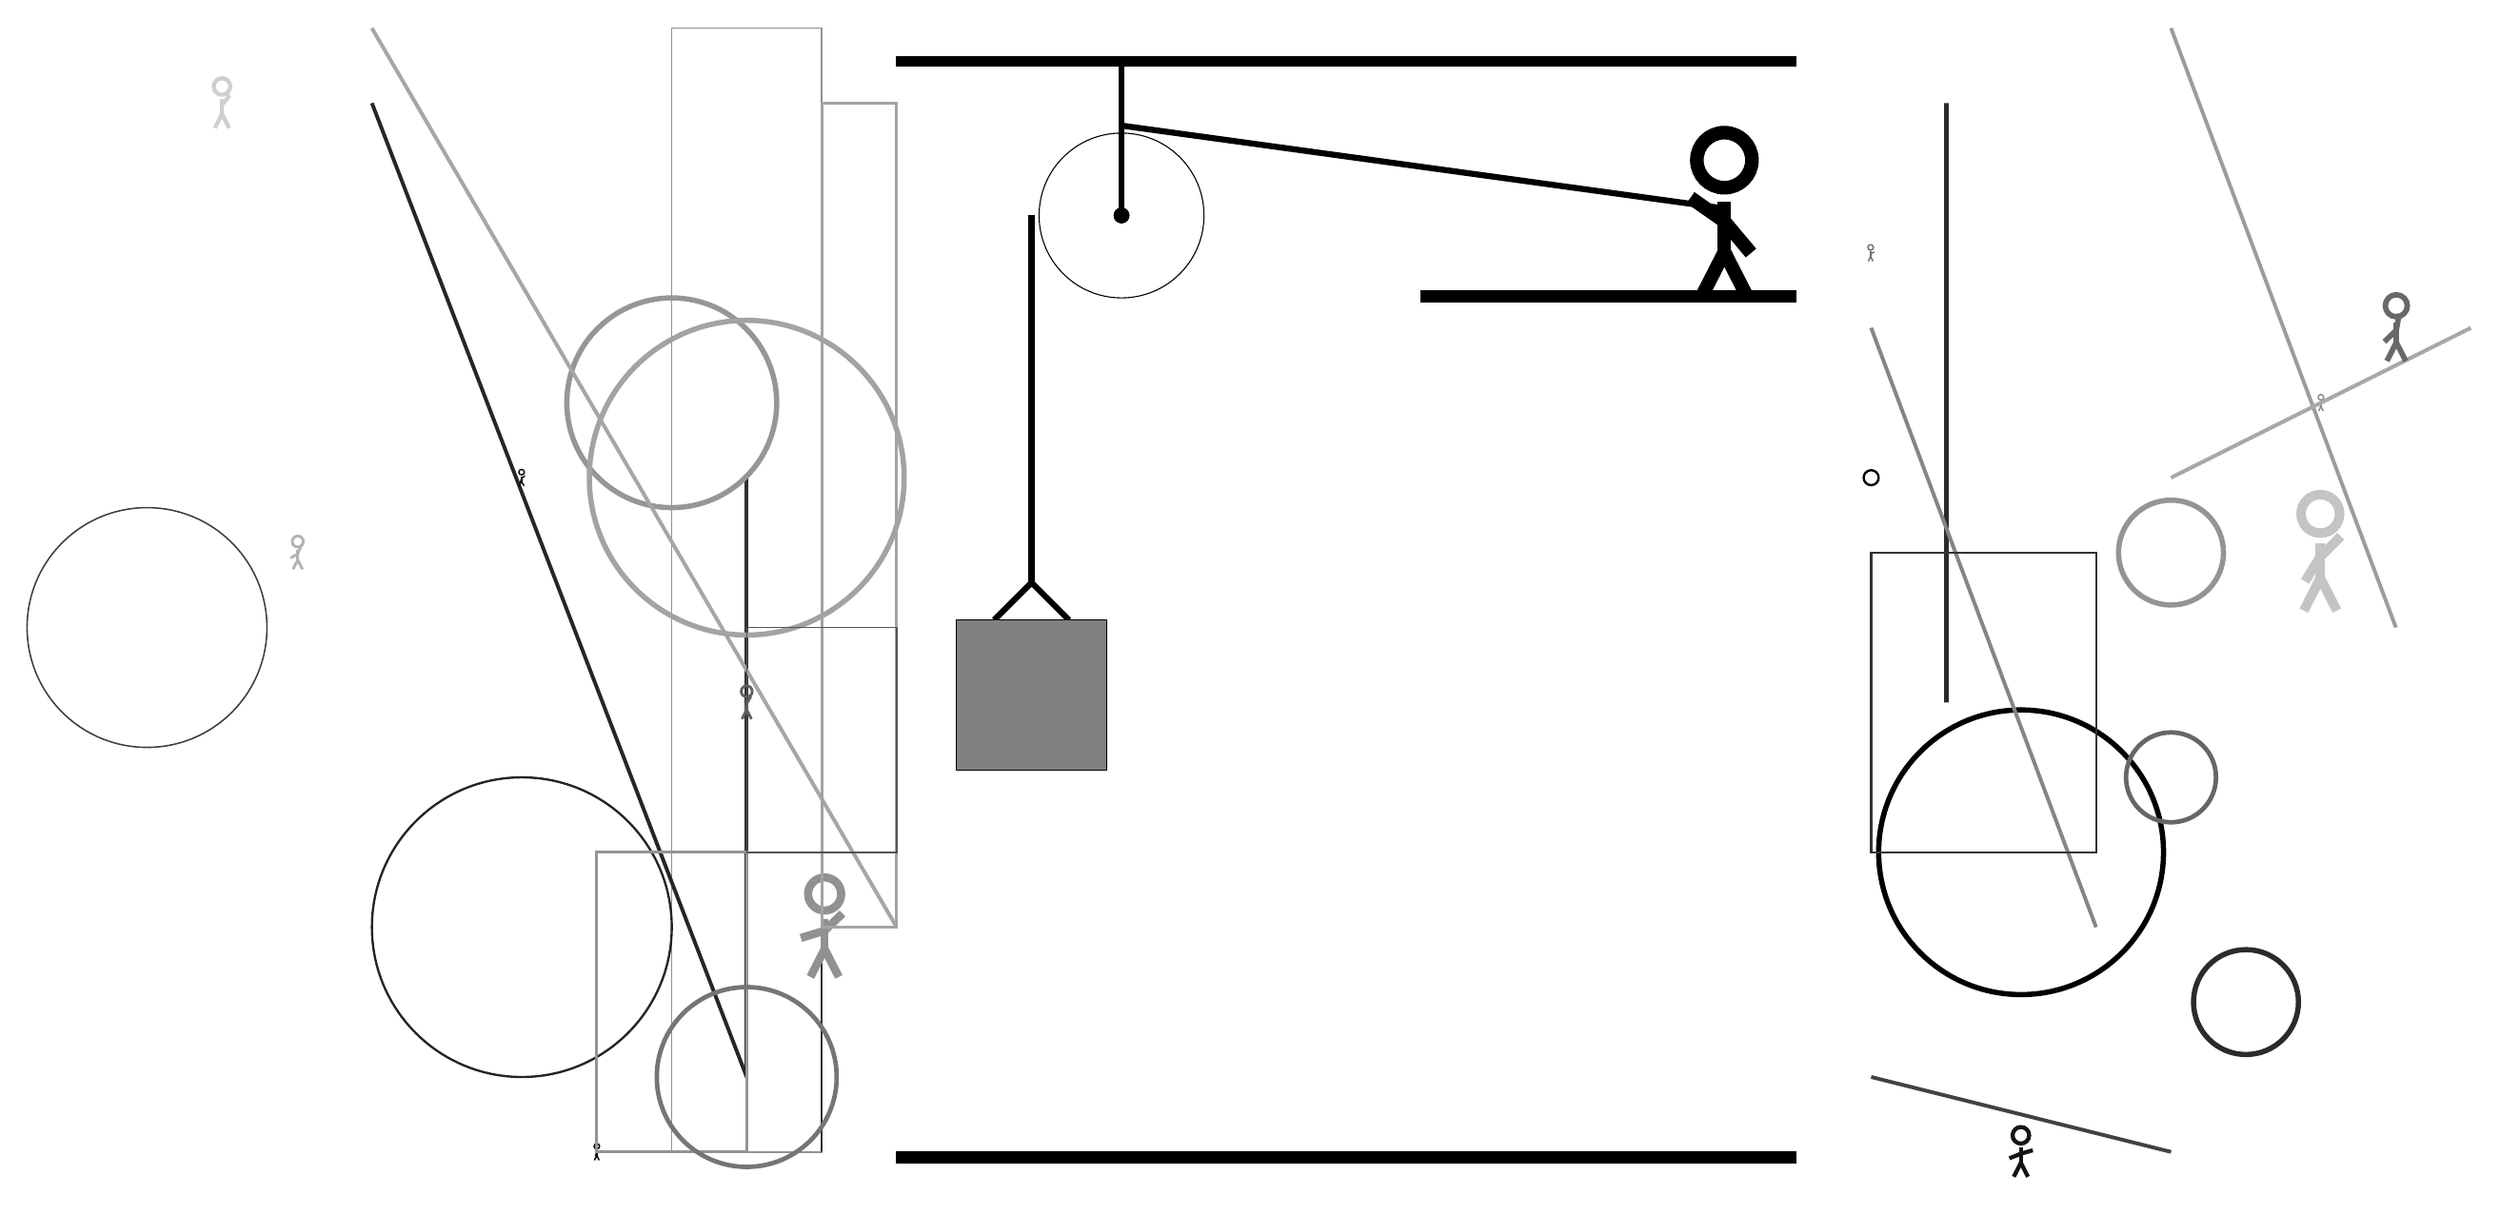
\begin{tikzpicture}
			%%%%% START %%%%%
			
			\draw[fill=black] (-2, 11.5) rectangle (10, 11.625);
			
			\draw (1, 9.5) circle (1.1);
			\draw[fill=black] (1, 9.5) circle (0.1);
			\draw[line width=0.8mm] (1, 11.5) -- (1, 9.5);
			
			\draw[line width=0.8mm](-0.7, 4.1) --  (-0.2, 4.6) -- (0.3, 4.1);
			\draw[fill=black!50] (-1.2, 4.1) rectangle (0.8, 2.1);
			
			\draw[line width=0.8mm](-0.2, 9.5) -- (-0.2, 4.6);
			\centerarc[line width=0.8mm](1, 9.5)(90:180:1.2000000000000002)
			\draw[line width=0.8mm](1, 10.7) -- (9, 9.6);
			
			\draw[line width=0.2mm, color=black!43] (-3, -3) rectangle (-5, 12);
			
			\draw [line width=0.7mm, color=black!42](15, 5) circle (0.7);
			\draw [line width=0.2mm, color=black!75](-12, 4) circle (1.6);
			\draw [line width=0.3mm, color=black!100](11, 6) circle (0.1);
			
			\draw[line width=0.3mm, color=black!81] (-3, -3) rectangle (-3, 3);
			\draw [line width=0.7mm, color=black!100](13, 1) circle (1.9);
			
			\draw[line width=0.5mm, color=black!39](15, 12) -- (18, 4);
			
			\node[line width=0.2mm, color=black!99] at (-6, -3) {\Strichmaxerl[1][69][83]};
			\draw[line width=0.6mm, color=black!83] (12, 11) rectangle (12, 3);
			\node[line width=0.6mm, color=black!23] at (17, 5) {\Strichmaxerl[7][58][45]};
			\draw[line width=0.5mm, color=black!81] (-4, 6) rectangle (-4, -2);
			
			\node[line width=0.4mm, color=black!43] at (-3, 0) {\Strichmaxerl[6][17][44]};
			\draw[line width=0.5mm, color=black!85](-4, -2) -- (-9, 11);
			
			\draw[line width=0.5mm, color=black!48](14, 0) -- (11, 8);
			\draw [line width=0.7mm, color=black!41](-5, 7) circle (1.4);
			\draw [line width=0.7mm, color=black!83](16, -1) circle (0.7);
			\draw [line width=0.3mm, color=black!86](-7, 0) circle (2.0);
			\draw[line width=0.3mm, color=black!80] (11, 5) rectangle (14, 1);
			\node[line width=0.2mm, color=black!97] at (-7, 6) {\Strichmaxerl[1][74][38]};
			\draw[line width=0.4mm, color=black!42] (-4, 1) rectangle (-6, -3);
			\draw[line width=0.5mm, color=black!35](-2, 0) -- (-9, 12);
			\node[line width=0.4mm, color=black!19] at (-11, 11) {\Strichmaxerl[3][90][51]};
			
			\draw [line width=0.7mm, color=black!36](-4, 6) circle (2.1);
			\node[line width=0.6mm, color=black!62] at (-4, 3) {\Strichmaxerl[2][81][60]};
			\draw[line width=0.5mm, color=black!74](15, -3) -- (11, -2);
			\node[line width=0.4mm, color=black!46] at (17, 7) {\Strichmaxerl[1][82][55]};
			\draw[line width=0.4mm, color=black!36] (-2, 11) rectangle (-3, 0);
			\node[line width=0.7mm, color=black!92] at (13, -3) {\Strichmaxerl[3][22][16]};
			
			\node[line width=0.2mm, color=black!30] at (-10, 5) {\Strichmaxerl[2][31][67]};
			
			\draw [line width=0.6mm, color=black!60](15, 2) circle (0.6);
			\draw[line width=0.5mm, color=black!34](15, 6) -- (19, 8);
			
			\node[line width=0.3mm, color=black!57] at (11, 9) {\Strichmaxerl[1][83][23]};
			\draw [line width=0.6mm, color=black!54](-4, -2) circle (1.2);
			\node[line width=0.5mm, color=black!59] at (18, 8) {\Strichmaxerl[4][44][80]};
			
			\draw[line width=0.2mm, color=black!67] (-4, 1) rectangle (-2, 4);
			
			\node at (9, 9.5) {\Strichmaxerl[10][-35][-50]};
			\draw[fill=black] (5, 8.5) rectangle (10, 8.35);
			
			\draw[fill=black] (-2, -3) rectangle (10, -3.15);
			
			%%%%% END %%%%%
		\end{tikzpicture}
	\end{figure}	
\end{document}